\documentclass[%11pt,
  use style = classical,
  scroll,
]{Q-A}

\def\PackageVersion{2023/11/01}
\def\PackageSubVersion{}

\newcommand{\QApackage}{{\normalfont\textsf{Q-A}}}


\title{\QApackage{}\\\smallskip\itshape Typesetting Q\&A-style conversation made easier}
\author{Jinwen XU}
% \thanks{Corresponding to: \texttt{\QApackage{}~\PackageVersion\PackageSubVersion}}
\date{\TheDate{\PackageVersion}[only-year-month], in Paris}


\newcommand{\meta}[1]{$\langle${\normalfont\itshape#1}$\rangle$}
\def\textcolon{:}
\def\texteqsign{=}
\def\textbacktick{`}
\def\textast{*}
\def\textsharp{\#}


\begin{document}

\maketitle

"
  Corresponding to: {\normalfont\texttt{\QApackage{}~\PackageVersion\PackageSubVersion}}.


##+ {Introduction}

?
  What is this?

:
  \QApackage{} is a \LaTeX{} document class for you to typeset Q\&A-style conversation. It turns a simple pure text Q\&A dialog like this:

  == {code/QA-doc-code-sample-content.tex}

  into a carefully designed document like this:

  \begin{center}
    \fbox{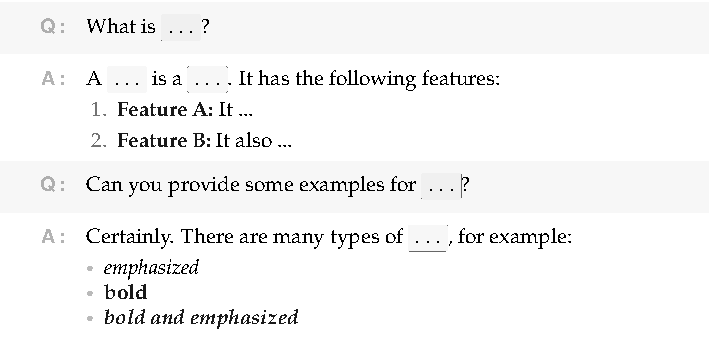
\includegraphics[width=.67\textwidth]{code/QA-doc-code-sample-content-result.pdf}}
  \end{center}


##+ {Preparation}

?
  That is nice. How can I use it? Is there anything that needs to be prepared?

:
  You should make sure that this document class is properly installed.

  If you are using TeX Live 2024 or newer, or the most recent version of MikTeX, then this package should already be included, and you don't need to do anything.

  Otherwise, you need to check for package update to see if you can receive it. In case not, you can always go to \href{https://ctan.org/pkg/Q-A}{the CTAN page} to download the `.zip` file with all related files included.


##+ {Usage}

?
  Now that I have successfully installed it, could you propose an example of usage?

:
  Of course. A typical document looks like this:

  == [latex] {code/QA-doc-code-sample-document.tex}

  The available class options include:
  \begin{itemize}
    \item `scroll`: turns the scroll mode on, which generates a single-page pdf similar to a long screenshot. It is recommended to use this option if your document contains some large piece of code.
    \item `use theme = \meta{theme}`: use the selected theme, available choices include: `default` (like the current document), `ChatGPT-light` and `ChatGPT-dark` (see the demo documents).
    \item Font size options such as `11pt`, `12pt`.
  \end{itemize}

?
  What about the main content?

:
  You have already seen an example of the main content. As you might have noticed, there are several syntaxes. Let me explain.

  [Questions (Q), Answers (A), and Narrations (N)]
  \begin{itemize}
    \item A question begins with the prefix `Q:` or `?`.
    \item An answer begins with the prefix `A:` or `:`.
    \item A narration begins with the prefix `N:` or `"`.
  \end{itemize}
  >>> Note that this depends on the current language. The prefixes `?`, `:` and `"` being universal, yet~—
  \begin{itemize}
    \item for French, it is Q\&R\&N, thus the alphabetical prefixes become `Q:`, `R:` and `N:`;
    \item for German, it is F\&A\&E, thus the alphabetical prefixes become `F:`, `A:` and `E:`;
    \item for Italian, it is D\&R\&N, thus the alphabetical prefixes become `D:`, `R:` and `N:`;
    \item for Portuguese and Brazilian, it is P\&R\&N, thus the alphabetical prefixes become `P:`, `R:` and `N:`;
    \item for Russian, it is B\&O\&P, thus the alphabetical prefixes become `B:`, `O:` and `P:`;
    \item for Spanish, it is P\&R\&N, thus the alphabetical prefixes become `P:`, `R:` and `N:`;
    \item for simplified Chinese, it is also possible to use the prefix `问:` for questions, `答:` for answers, and `注:` for narrations; similarly for traditional Chinese;
    \item for Chinese or Japanese, it is also possible to use the prefix `?` for questions, `:` for answers, and `“`, `”` or `「` for narrations.
  \end{itemize}

  [Emphasize and Bold]
  \begin{itemize}
    \item Use `\textast\meta{text}\textast` to emphasis `\meta{text}`.
    \item Use `\textast\textast\meta{text}\textast\textast` to make `\meta{text}` into boldface.
    \item Use `\textast\textast\textast\meta{text}\textast\textast\textast` to combine the previous effects.
  \end{itemize}

  [Emphasized Enumeration]
  An emphasized enumeration, like the current line, is marked by `[\meta{text}]` at the beginning, where `\meta{text}` is the text to be emphasized.
  >>> If you wish to restart the numbering from \( 1 \), write an asterisk after the final bracket: `[\meta{text}]\textast`.

  [Sections]
  \begin{itemize}
    \item You may start a new (*unnumbered*) ---
    \begin{itemize}
      \item section, via `\textsharp\textsharp{} \{\meta{section title}\}`;
      \item subsection, via `\textsharp\textsharp\textsharp{} \{\meta{subsection title}\}`;
      \item subsubsection, via `\textsharp\textsharp\textsharp\textsharp{} \{\meta{subsubsection title}\}`;
    \end{itemize}
    \item If you wish to use the *numbered* version, write `\textsharp\textsharp+`, `\textsharp\textsharp\textsharp+` and `\textsharp\textsharp\textsharp\textsharp+` instead.
  \end{itemize}

  [Input/Include Files]
  \begin{itemize}
    \item Use `\textcolon\textcolon{} \{\meta{file name}\}` to input a file.
    \item Use `\textcolon\textcolon\textcolon{} \{\meta{file name}\}` to include a file.
  \end{itemize}

  [Code]
  Due to the current implementation of this document class, it is unfortunate that you cannot directly insert source code in your document. There are some workarounds, though.
  \begin{itemize}
    \item For *displayed* code, stored the code into a separate file, and then use `\texteqsign\texteqsign{} \{\meta{file name}\}` to print it. You may also use an optional argument like `\texteqsign\texteqsign{} [\meta{language}] \{\meta{file name}\}` to select the language of your code.
    \item For *inline* code, you may simply write it between two backticks `\textbacktick\meta{code}\textbacktick`, similar to the Markdown syntax. However, be aware that special characters need to be escaped, for example, `\textbackslash` should be written as `\textbackslash textbackslash`, `\{` should be written as `\textbackslash\{`, `\%` should be written as `\textbackslash\%`, etc.
  \end{itemize}

  And don't forget that you are still using \LaTeX, so images, tables and lists can be written as usual.

?
  I see. Is there anything else for me to be careful about?

:
  Glad that you asked. Here are several things that should be taken care of:
  \begin{itemize}
    \item A question, answer or narration should always begin in a new paragraph.
    \item An emphasized enumeration should also begin in a new paragraph.
    \item Likewise, a `section`/`subsection`/`subsubsection` should be placed in a separate paragraph.
    \item Input or inclusion of files should also be operated in a separate paragraph.
    \item For emphasizing and bolding the text, it would be necessary to separate the asterisks with~`\{\}` in some special cases: `\textast\textast like\textast\textast\{\}\textast\textast\textast this\textast\textast\textast\{\}\textast one\textast`.
  \end{itemize}


##+ {Customization}

?
  Now that we have learned the basic usage, I would like to know more. Can I customize the interface to suit my preferences, for instance?

:
  Certainly. Apart from using themes via class option, you may also change the identifiers and the labels for each role in the conversation.

  [Changing itentifiers]
  Instead of the default identifiers, such as `?` for questions, you may also use your preferred one. This can be done via the use of `\backslash QASetTypePrefix` in the preamble of your document.
  \begin{itemize}
    \item Use `\backslash QASetTypePrefix\{Q\}\{\meta{identifiers}\}` to set the identifiers for questions.
    \item Use `\backslash QASetTypePrefix\{A\}\{\meta{identifiers}\}` to set the identifiers for answers.
    \item Use `\backslash QASetTypePrefix\{N\}\{\meta{identifiers}\}` to set the identifiers for narrations.
  \end{itemize}
  Here, \meta{identifier} is a comma list of your specified identifiers. For example, the default identifier for narrations is preset via `\backslash QASetTypePrefix\{N\}\{N:,",“,”,「\}`.
  \QAnote{Note that, due to its implementation, the identifier cannot contain comma `,` in it. If you wish to use an identifier that contains a comma, you may use `\backslash QAAddTypePrefix` instead, which only adds *one* identifier per use.}
  \QAnote{Note also that, the identifiers are *reset* upon changing of language. Thus, you need to put your setting into the corresponding language configuration, for example, via `\backslash AddLanguageSetting[\meta{language name}]\{\meta{settings}\}`}

  [Changing labels]
  You may also change the labels. For example, from the text \textquote{Q:} to a logo icon. This can be done via the use of `\backslash SetLogoCode` in the preamble of your document.
  \begin{itemize}
    \item Use `\backslash SetLogoCode\{Q\}\{\meta{logo code}\}` to set the labels for questions.
    \item Use `\backslash SetLogoCode\{A\}\{\meta{logo code}\}` to set the labels for answers.
  \end{itemize}
  Here, \meta{logo code} is the actual code for displaying the corresponding label. For example, the default label for questions is preset via `\backslash SetLogoCode\{Q\}\{\textbackslash textbf\{Q\textbackslash,:\}\}`.
  >>> In the demo document, you can find an example on how to use this command to specify a logo for each role in the conversation.


##+ {Known Issues}

?
  Is there any known issue with this document class?

:
  Unfortunately, yes `:(`.

  Below is a list of known issues:

  \begin{itemize}
    \item Currently, the code highlight is done by the package `listings`. Due to its own limitations, the result is still far from satisfactory. Using `minted` instead could improve the situation, but this would require `-shell-escape` and some external tweaking, thus it would still take some effort to make it work with the current document class.
    \item Due to the current implementation, though it is already possible to automatically adopt the identifiers and labels for supported languages, you still need to use the identifiers `Q`, `A` and `N` when setting them.
    \item Since the text is in fact already put into a list, the level of lists might be slightly messed up, which could sometimes lead to wrong spacing.
  \end{itemize}


##+ {Get Support}

?
  What should I do if I encounter any problem?

:
  If you run into any issues or have ideas for improvement, feel free to discuss on:
  \begin{center}
      \url{https://github.com/Jinwen-XU/Q-A/issues}
  \end{center}
  or email me via \href{mailto:ProjLib@outlook.com}{\texttt{ProjLib@outlook.com}}.


\vspace{3\baselineskip}

% ---

% "
%   Below is the code of the current document.

%   == [latex] {\jobname.tex}

\end{document}
